\begin{figure}[hbt!]
    \begin{subfigure}[b]{0.5\textwidth}
        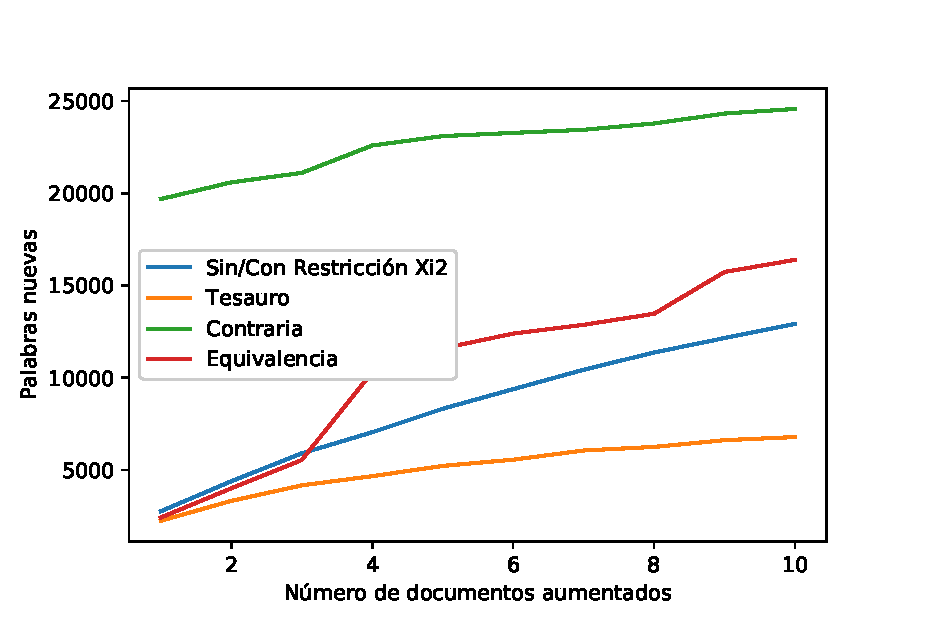
\includegraphics[width=\textwidth]{sections/figures/pos_plot.eps}
        \caption{Depresión: Clase positiva}
    \end{subfigure}
    \hfill
    \begin{subfigure}[b]{0.5\textwidth}
        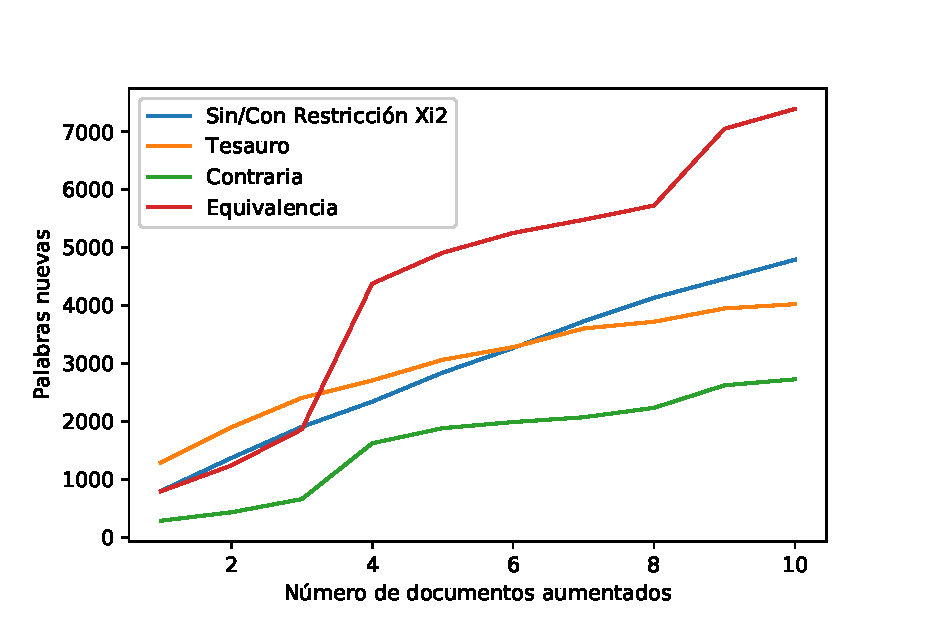
\includegraphics[width=\textwidth]{sections/figures/both_plot_1.eps}
        \caption{Depresion: Ambas clases}
    \end{subfigure}
    \hfill
    
    \begin{subfigure}[b]{0.5\textwidth}
        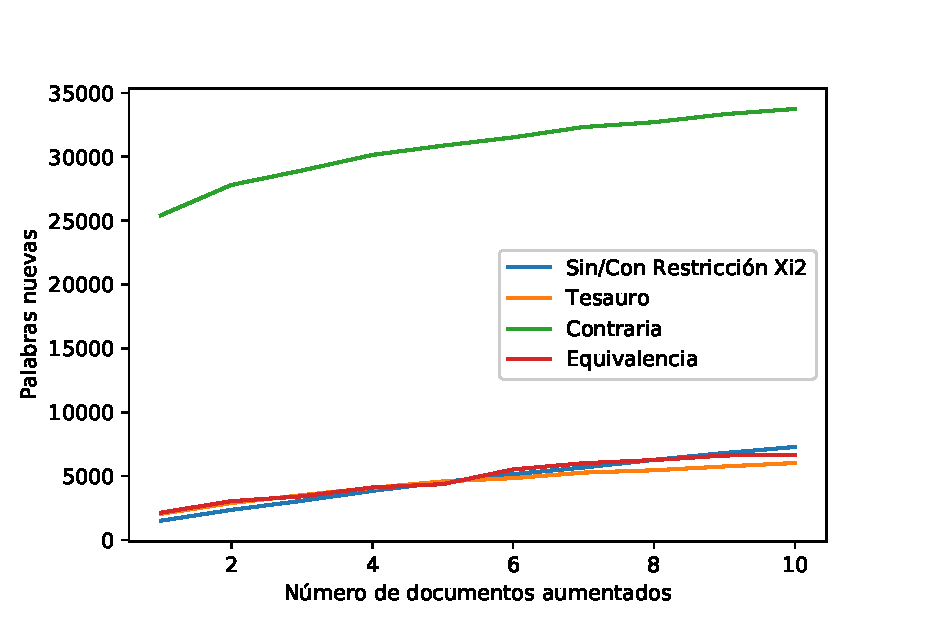
\includegraphics[width=\textwidth]{sections/figures/pos_plot_anox.eps}
        \caption{Anorexia: Clase positiva}
    \end{subfigure}
    \hfill
    \begin{subfigure}[b]{0.5\textwidth}
        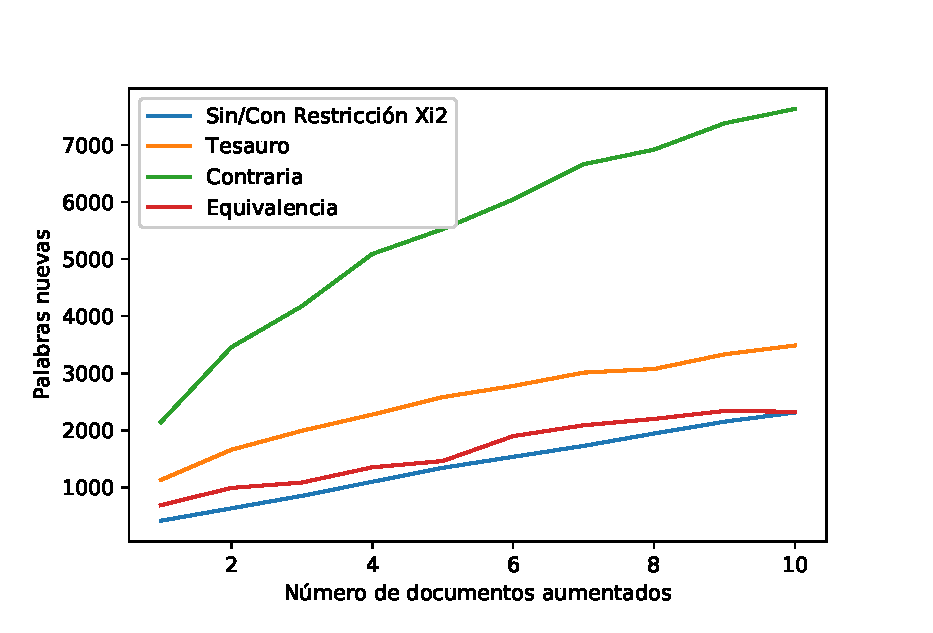
\includegraphics[width=\textwidth]{sections/figures/both_plot_anox.eps}
        \caption{Anorexia: Ambas clases}
    \end{subfigure}
    
    
    \caption{Relación entre el numero de documentos aumentados y el vocabulario nuevo agregado.}
    \label{fig:aumento_vocab_dep}
\end{figure}